\begin{lstlisting}
Section 6.2:  9, 10, 11, 12,  16(ed7: 14)
\end{lstlisting}
\begin{exercise}
\begin{figure}[H]
\centering
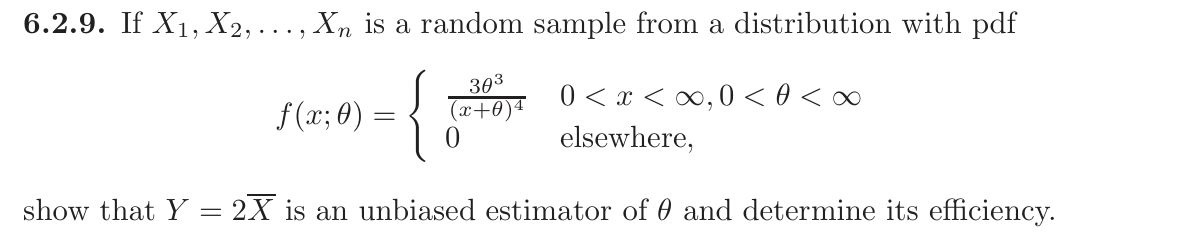
\includegraphics[width=\textwidth]{hw8-2025042517.png}
% \caption{}
\label{}
\end{figure}
\end{exercise}
\begin{proof}
\begin{equation}
\mathbb{E}(Y)=\mathbb{E}(2\overline{X})=2\mathbb{E}(X_1)=2\int_{0}^{\infty} xf(x;\theta) \, \mathrm{d}x =2\int_{0}^{\infty} \frac{3\theta^{3}x}{(x+\theta)^{4}} \, \mathrm{d}x =\theta
\label{c462b0}
\end{equation}

So $Y$ is an unbiased estimator of $\theta$.
\[
\frac{ \partial \log f(X;\theta) }{ \partial \theta }=\frac{ \partial   }{ \partial \theta } \log \frac{3\theta^{3}}{(X+\theta)^{4}}=\frac{ \partial   }{ \partial \theta } (3\log\theta-4\log(X+\theta)+\log3)=\frac{3}{\theta}-\frac{4}{X+\theta}
\]
\[
\frac{ \partial^2 \log f(X;\theta) }{ \partial \theta ^2 } =-\frac{3}{\theta^{2}}+\frac{4}{(X+\theta)^2}
\]
The fisher information is
\[
\begin{aligned}
I(\theta) & =-\mathbb{E}\left[ -\frac{9}{\theta^{2}}+\frac{4}{(X+\theta)^2} \right]=\frac{9}{\theta^{2}}-4\cdot \mathbb{E}\left[ \frac{1}{(X+\theta)^2} \right] \\
 & =\frac{3}{\theta^{2}}-4\int_{0}^{\infty} \frac{1}{(x+\theta)^2}\cdot\frac{3\theta^{3}}{(x+\theta)^{4}} \, \mathrm{d}x  \\
 & =\frac{3}{\theta^{2}}-\frac{12}{5\theta^{2}}=\frac{3}{5\theta^{2}}
\end{aligned}
\]
The Rao–Cramér lower bound in this case is
\[
\frac{1}{nI(\theta)}=\frac{5\theta^{2}}{3n}
\]
The variance of $Y$ is
\[
\begin{aligned}
\mathrm{Var}(Y) & =\mathrm{Var}(2\overline{X})=\frac{4}{n}\mathrm{Var}(X_1) \\
 & =\frac{4}{n}\left( \underbrace{ \int_{0}^{\infty} \frac{3\theta^{3}x^2}{(x+\theta)^{4}} \, \mathrm{d}x }_{ =\mathbb{E}(X_1^2) } -\left[ \underbrace{ \int_{0}^{\infty} \frac{3\theta^{3}x}{(x+\theta)^{4}} \, \mathrm{d}x }_{ =\mathbb{E}(X_1) } \right]^2 \right)  \\
 & =\frac{4}{n}\left[ \theta^{2}-\left( \frac{\theta}{2} \right)^2 \right] \\
 & =\frac{3\theta^{2}}{n}
\end{aligned}
\]
The efficiency is
\[
e(Y)=\frac{1}{nI(\theta)\cdot \mathrm{Var}(Y)}=\frac{5}{9} 
\]
\end{proof}

\begin{exercise}
\begin{figure}[H]
\centering
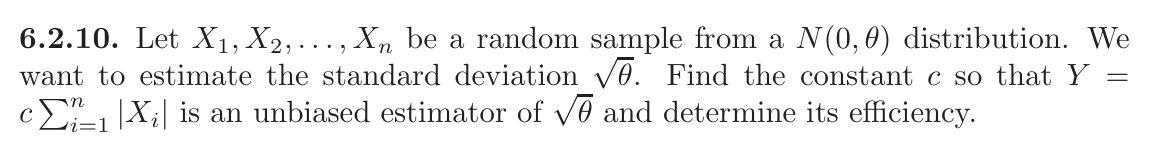
\includegraphics[width=\textwidth]{1-hw8-2025042517.png}
% \caption{}
\label{}
\end{figure}
\end{exercise}
\[
\begin{aligned}
\mathbb{E}[Y] & =c\sum_{i=1}^{n} \mathbb{E}[\lvert X_i \rvert ]=c\sum_{i=1}^{n}\frac{1}{\sqrt{ 2\pi\theta }}\int_{-\infty}^{\infty} \lvert x \rvert \cdot \exp\left(- \frac{x^2}{2\theta} \right) \, \mathrm{d}x \\
 & =2\sqrt{ \frac{\theta}{2\pi} }\cdot c\sum_{i=1}^{n} \int_{0}^{\infty} e^{- y } \, \mathrm{d}y  \\
 & =2\sqrt{ \frac{\theta}{2\pi} }\cdot cn
\end{aligned}
\]
Let $\mathbb{E}[Y]=\sqrt{ \theta }$ then $c=\frac{\sqrt{ 2\pi }}{2n}$.
\[
\frac{ \partial \log f(X;\theta) }{ \partial \theta } =\frac{ \partial   }{ \partial \theta }\left( -\frac{X^2}{2\theta}-\log \sqrt{ 2\pi \theta } \right) =\frac{X^2}{2\theta^{2}}-\frac{1}{2\theta}
\]
\[
\frac{ \partial^2 \log f(X;\theta) }{ \partial \theta ^2 } =-\frac{X^2}{\theta^{3}}+\frac{1}{2\theta^{2}}
\]
\[
I(\theta)=\mathbb{E}\left[ -\frac{ \partial^2 \log f(X;\theta) }{ \partial \theta ^2 }  \right]=\frac{1}{\sqrt{ 2\pi\theta }}\int_{-\infty}^{\infty} \left( \frac{x^2}{\theta^{3}}-\frac{1}{2\theta^{2}} \right)e^{ -x^2/2\theta } \, \mathrm{d}x =\frac{1}{2\theta^{2}}
\]
\[
\begin{aligned}
\mathrm{Var}(Y) & =\mathrm{Var}\left( \frac{\sqrt{ 2\pi }}{2n}\sum_{k=1}^{n} \lvert X_k \rvert  \right)=\frac{\pi}{8n}\mathrm{Var}(\lvert X_1 \rvert ) \\
 & =\frac{\pi}{2n}(\mathbb{E}(X_1^2)-(\mathbb{E}[\lvert X_1 \rvert ])^2) \\
 & =\frac{\pi}{2n}\left( \frac{1}{\sqrt{ 2\pi \theta }}\int_{-\infty}^{\infty} x^2e^{ -x^2/2\theta } \, \mathrm{d}x  -\left( \frac{1}{\sqrt{ 2\pi \theta }}\int_{-\infty}^{\infty} \lvert x \rvert e^{ -x^2/2\theta } \, \mathrm{d}x  \right)^2\right) \\
 & =\frac{\pi  \left(\theta -\frac{2 \theta }{\pi }\right)}{2 n}=\frac{\pi-2}{2n}\theta
\end{aligned}
\]
The efficiency is
\[
e(Y)=\frac{1}{nI(\sqrt{ \theta })\cdot \mathrm{Var}(Y)}=\frac{1}{\pi-2}
\]
\begin{exercise}
\begin{figure}[H]
\centering
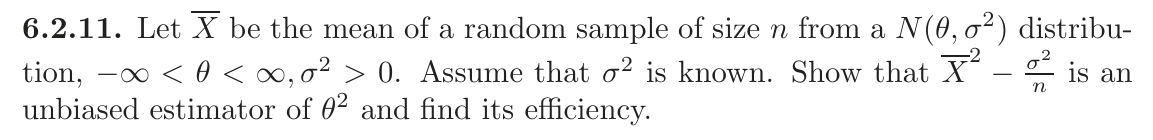
\includegraphics[width=\textwidth]{2-hw8-2025042517.png}
% \caption{}
\label{}
\end{figure}
\end{exercise}
\[
\overline{X}=\frac{1}{n}\sum_{k=1}^{n} X_k\sim N\left( \theta,\frac{\sigma^{2}}{n} \right)
\]
\[
\begin{aligned}
\mathbb{E}\left[ \overline{X}^2-\frac{\sigma^{2}}{n} \right] & =\mathbb{E}[\overline{X}^2]-\frac{\sigma^{2}}{n} \\
& =\frac{1}{\sqrt{ 2\pi }\cdot \sigma/\sqrt{ n }}\int_{-\infty}^{\infty} x^2\cdot \exp \left\{  -\frac{(x-\theta)^2}{2\sigma^{2}/n}  \right\} \, \mathrm{d}x -\frac{\sigma^{2}}{n}  \\
& =\frac{\theta ^2 n+\sigma ^2}{\sqrt{n} \sigma  \sqrt{\frac{n}{\sigma ^2}}}-\frac{\sigma^{2}}{n}  \\
& =\theta^{2}
\end{aligned}
\]
Thus $\overline{X}^2-\frac{\sigma^{2}}{n}$ is unbiased estimator of $\theta^{2}$.
\[
\begin{aligned}
\frac{ \partial \log f(X;\theta) }{ \partial \theta }  & =\frac{ \partial   }{ \partial \theta } \log\left( \frac{1}{\sqrt{ 2\pi }\sigma}\exp \left\{  -\frac{(X-\theta )^2}{2\sigma^{2}}  \right\} \right) \\
 & =\frac{ \partial   }{ \partial \theta } \left[ -\frac{(X-\theta)^2}{2\sigma^{2}}-\log(\sqrt{ 2\pi  }\sigma) \right] \\
 & =\frac{1}{\sigma^{2}}(X-\theta)
\end{aligned}
\]
\[
\frac{ \partial^2 \log f(X;\theta) }{ \partial \theta ^2 } =\frac{ \partial   }{ \partial \theta } \left( \frac{1}{\sigma^{2}}(X-\theta) \right)=-\frac{1}{\sigma^{2}}
\]
\[
I(\theta)=\mathbb{E}\left[ -\frac{ \partial^2 \log f(X;\theta) }{ \partial \theta ^2 }  \right]=\frac{1}{\sigma^{2}}
\]
\[
\begin{aligned}
\mathrm{Var}\left( \overline{X}^2-\frac{\sigma^{2}}{n} \right) & =\mathrm{Var}(\overline{X}^2)=\mathbb{E}[\overline{X}^{4}]-(\mathbb{E}[\overline{X}^2])^2 \\
 & =\frac{1}{\sqrt{ 2\pi }\sigma/\sqrt{ n }}\int_{-\infty}^{\infty} x^{4}e^{ -(x-\theta)^2/(2\sigma^{2}/n) } \, \mathrm{d}x  \\
 & \quad -\left[ \frac{1}{\sqrt{ 2\pi }\sigma/\sqrt{ n }}\int_{-\infty}^{\infty} x^{2}e^{ -(x-\theta)^2/(2\sigma^{2}/n) } \, \mathrm{d}x \right]^2 \\
 & =\frac{n^2\theta^{4}+6n\theta^{2}\sigma^{2}+3\sigma^{2}}{n^2}-\left( \frac{n\theta^{2}+\sigma^{2}}{n} \right)^2 \\
 & =\frac{4n\theta^{2}\sigma^{2}+2\sigma^{2}}{n^2}
\end{aligned}
\]
The efficiency is
\[
e\left( \overline{X}^2-\frac{\sigma^{2}}{n} \right)=\frac{1}{nI(\theta^{2})\cdot\mathrm{Var}\left( \overline{X}^2-\frac{\sigma^{2}}{n} \right)}=\frac{n}{4n\theta^{2}\sigma^{2}+2\sigma^{2}}
\]
\begin{exercise}
\begin{figure}[H]
\centering
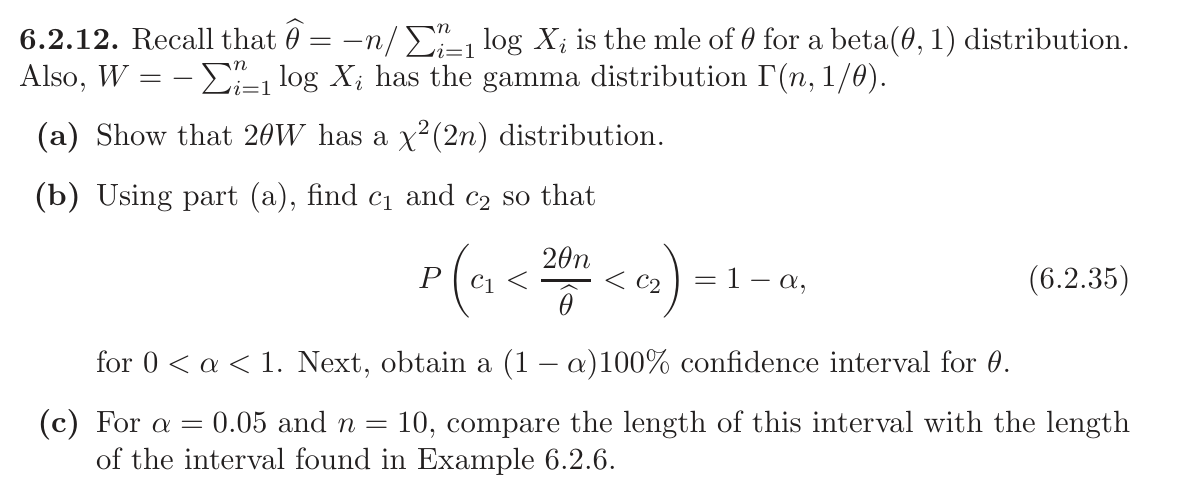
\includegraphics[width=\textwidth]{3-hw8-2025042517.png}
% \caption{}
\label{}
\end{figure}
\end{exercise}
(a)
We say $W \sim \Gamma(n, 1/\theta)$ if the pdf of $W$
\[
f_{W}(x)=\frac{1}{\Gamma(n) (1/\theta)^n} x^{n-1} e^{-\theta x }=\frac{\theta^{n}}{(n-1)!} x^{n-1} e^{-\theta x } \quad 0<x<\infty
\]
The characteristic function of $\Gamma(a, \beta)$ is
\[
\begin{aligned}
\varphi(t) & =E\left[e^{i X t}\right]=\int_0^{\infty} e^{i x t} \cdot \frac{1}{\Gamma(\alpha) \beta^\alpha} x^{\alpha-1} e^{-x / \beta} d x \\
& =\frac{1}{\Gamma(\alpha) \beta^\alpha} \int_0^{\infty} x^{\alpha-1} e^{(i t-1 / \beta) x} d x \\
& =(1-i \beta t)^{-\alpha}
\end{aligned}
\]
Then
\[
\varphi_{W}(t)=(1-i\theta ^{-1}t)^{-n}
\]
\[
\varphi_{2\theta W}(t)=\mathbb{E}[\exp \{ it\cdot2\theta W \}]=\varphi(2\theta t)=(1-2it)^{-n}
\]
Thus $2\theta W\sim \chi^{2}(2n)$.

(b)
\[
\mathbb{P}\left( c_1<\frac{2\theta n}{\widehat{\theta}}<c_2 \right)=\mathbb{P}(c_1<2\theta W<c_2)
\]
Let $c_1=0$, $c_2=\chi^{2}_{2n,\alpha}$, where $\mathbb{P}(X>\chi^{2}_{2n,\alpha})=\alpha$ for $X\sim \chi^{2}(2n)$.

(c)
When $\alpha=0.05, n=10$, then $c_2=\chi^{2}_{2n,\alpha}=31.410$. The confidence interval is
\[
(0,31.410)
\]
\begin{exercise}
\begin{figure}[H]
\centering
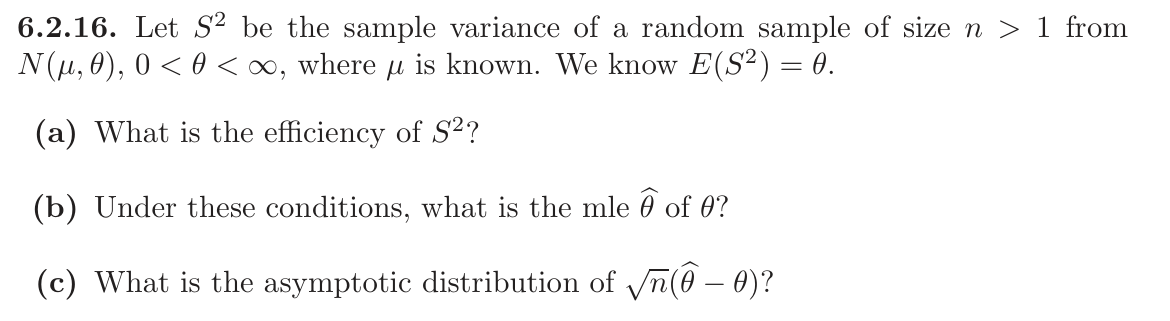
\includegraphics[width=\textwidth]{4-hw8-2025042517.png}
% \caption{}
\label{}
\end{figure}
\end{exercise}
(a)
\[
S^2=\frac{1}{n-1}\sum_{k=1}^{n} (X_k-\overline{X})^2=\frac{1}{n-1}\sum_{k=1}^{n} X_k^2-\frac{n}{n-1}\mu^{2}
\]
\[
\begin{aligned}
\frac{ \partial \log f(X;\theta) }{ \partial \theta }  & =\frac{ \partial   }{ \partial \theta } \log\left( \frac{1}{\sqrt{ 2\pi \theta }}\exp \left\{  -\frac{(X-\mu)^2}{2\theta}  \right\} \right) \\
 & =\frac{ \partial   }{ \partial \theta } \left( -\frac{(X-\mu)^2}{2\theta}-\log \sqrt{ 2\pi\theta } \right) \\
 & =\frac{(X-\mu)^2}{2\theta^{2}}-\frac{1}{2\theta} 
\end{aligned}
\]
\[
\frac{ \partial^2 \log f(X;\theta) }{ \partial \theta ^2 }=\frac{ \partial   }{ \partial \theta } \left[ \frac{(X-\mu)^2}{2\theta^{2}}-\frac{1}{2\theta} \right]=-\frac{(X-\mu)^2}{\theta^{3}}+\frac{1}{2\theta^{2}}
\]
\[
I(\theta)=\mathbb{E}\left( -\frac{ \partial^2 \log f(X;\theta) }{ \partial \theta ^2 }  \right)=-\frac{1}{2\theta^{2}}+\frac{1}{\theta^{3}}\underbrace{ \mathbb{E}[(X-\mu)^2] }_{ =\theta }=\frac{1}{2\theta^{2}}
\]
\[
\begin{aligned}
\mathrm{Var}(S^2) & =\mathrm{Var}\left( \frac{1}{n-1}\sum_{k=1}^{n} (X_k-\overline{X})^2 \right) \\
 & =\frac{1}{(n-1)^2}\sum_{k=1}^{n} \mathrm{Var}[(X_k-\overline{X})^2] \\
 & =\frac{1}{(n-1)^2}\sum_{k=1}^{n} (\mathbb{E}[(X_k-\overline{X})^{4}]-(\mathbb{E}[(X_k-\overline{X})^2])^2) \\
 & =\frac{1}{(n-1)^2}\sum_{k=1}^{n} (\mathbb{E}[(X_k-\mu)^{4}]-(\mathbb{E}[(X_k-\mu)^2])^2)  \\
 & =\frac{1}{(n-1)^2}\sum_{k=1}^{n} \left[ \underbrace{ \frac{1}{\sqrt{ 2\pi\theta }}\int_{-\infty}^{\infty} (x-\mu)^{4}e^{ -(x-\mu)^2/2\theta } \, \mathrm{d}x }_{ =3\theta^{2} }  -\left(\underbrace{  \frac{1}{\sqrt{ 2\pi\theta }}\int_{-\infty}^{\infty } (x-\mu)^2e^{ -(x-\mu)^2/2\theta } \, \mathrm{d}x   }_{ =\theta }\right)^2 \right] \\
 & =\frac{2n\theta^{2}}{(n-1)^2}
\end{aligned}
\]
The efficiency is
\[
e(\theta)=\frac{1}{nI(\theta)\mathrm{Var}(S^2)}=\frac{1}{n \cdot\frac{1}{2\theta^{2}}\cdot\frac{2n\theta^{2}}{(n-1)^2}}=\frac{(n-1)^2}{n^2}
\]
(b)
The log-likelihood function is
\[
\sum_{k=1}^{n} \log f(X_k;\theta)
\]
Let
\[
\frac{ \partial   }{ \partial \theta } \sum_{k=1}^{n} \log f(X_k;\theta)=\sum_{k=1}^{n} \frac{ \partial   }{ \partial \theta } \log f(X_k;\theta)=0
\]
i.e.
\begin{equation}
0=\sum_{k=1}^{n}\left[  \frac{(X_k-\mu)^2}{2\theta^{2}}-\frac{1}{2\theta}  \right]=\frac{1}{2\theta^{2}}\left( \sum_{k=1}^{n} X_k^2-n\mu^{2} \right)-\frac{n}{2\theta}
\label{51d91f}
\end{equation}

The solution of \cref{51d91f}, $\widehat{\theta}=\frac{1}{n}\left( \sum_{k=1}^{n}X_k^2 -n\mu^{2}\right)$, is the mle of $\theta$.
\[
\widehat{\theta}=\frac{1}{n}\sum_{k=1}^{n} (X_k-\overline{X})^2=\frac{n-1}{n}S^2
\]
(c)
\[
Y_n\coloneqq \sqrt{ n }(\widehat{\theta}-\theta)=\sqrt{ n }\left( \frac{n-1}{n}S^2 \right)-\sqrt{ n }\theta
\]
By Student's theorem,
\[
W\coloneqq (n-1)S^2/\theta \sim \chi^{2}(n-1)
\]
Then the characteristic function of $W$ is
\[
\varphi_{W}(t) =(1-2it)^{-(n-1)/2}
\]
The characteristic function of $Y$ is
\[
\begin{aligned}
\varphi_{Y_n}(t) & =\mathbb{E}[\exp \{ itY \}] \\
 & =\mathbb{E}\left[ \exp \left\{  it\cdot \sqrt{ n }\cdot\frac{n-1}{n}S^2-it\sqrt{ n }\theta  \right\} \right] \\
 & =e^{ -it\sqrt{ n }\theta }\cdot \mathbb{E}\left[ \frac{it\theta }{\sqrt{ n }}\cdot\frac{(n-1)S^2}{\theta} \right] \\
 & =e^{ -it\sqrt{ n }\theta }\cdot\varphi_{W}\left( \frac{t\theta }{\sqrt{ n }} \right) \\
 & =e^{ -it\sqrt{ n }\theta }\cdot\left( 1-\frac{2it\theta}{ \sqrt{ n }}  \right)^{-(n-1)/2} \\
 & =\exp \left\{  -it\sqrt{ n }\theta-\frac{n-1}{2}\log\left( 1-\frac{2it\theta}{\sqrt{ n }} \right)  \right\} \\
 & =\exp \left\{  -it\sqrt{ n }\theta +\frac{n-1}{2} \left( \frac{2it\theta}{ \sqrt{ n }}+\frac{1}{2}\cdot\left( \frac{2it\theta}{ \sqrt{ n }} \right)^2+o(n^{-1}) \right)\right\} \\
 & =\exp \left\{  -it\sqrt{ n }\theta+ it\sqrt{ n }\theta-\theta^{2}t^2+o(1) \right\} \\
 & =\exp \{ -\theta^{2}t^2+o(1) \} \\
 & \to \exp \{ -\theta^{2}t^2 \}
\end{aligned}
\]
By the inverse formula, the asymptotic pdf of $Y_n$ is
\[
\lim_{ n \to \infty } f_{Y_n}(x)=\frac{1}{2\pi}\int_{-\infty}^{\infty} e^{ -\theta^{2}t^2 }e^{ -itx } \, \mathrm{d}x =\frac{1}{\sqrt{ 2\pi }\cdot \sqrt{ 2 }\theta}\exp \left\{  -\frac{x^2}{2\cdot(\sqrt{ 2 }\theta)^2}  \right\}
\]
Thus $Y_n\sim N(0,2\theta^{2})$.
